\section{Planning in NLG} \label{sec:domains}

In this section, we present our planning domains: the sentence
generation domain and the instruction giving domain.


\subsection{Sentence generation as planning}

Sentence generation is the problem of computing, from a grammar and a
semantic representation, a single sentence that expresses this piece of
meaning.  This problem is traditionally split into several steps
\cite{reiter00building}.  In a first step, called \emph{sentence planning},
the semantic representation is first enriched with more information; for
instance, \emph{referring expressions}, which refer to individuals
that we want to talk about, are determined at this point. In a second
step, called \emph{surface realization}, this enriched representation is
then translated into a natural-language sentence, using the grammar.

In practice, the process of determining referring expressions typically
interacts with the realization step and so it turns out to be beneficial to
perform both of these steps together. This was the goal of the SPUD system
\cite{Stone2003a}, which performed both steps together using a top-down
generation algorithm based on tree-adjoining grammars \cite{joshi;etal1997}
whose lexical entries were equipped with semantic and pragmatic
information. Unfortunately, SPUD suffered from having to explore a huge
search space, and had to resort to a non-optimal greedy search strategy to
retain reasonable efficiency. 

%However, determining referring expressions and realization
%interact, so it would be beneficial to perform both steps together.
%This was the goal of the SPUD system \cite{Stone2003a}, which
%performed both steps together using a top-down generation algorithm
%based on tree-adjoining grammars \cite{joshi;etal1997} whose lexical
%entries were equipped with semantic and pragmatic information.
%Unfortunately, SPUD suffered from having to explore a huge search
%space, and had to resort to a non-optimal greedy search strategy to
%retain reasonable efficiency.

\begin{figure}
  \centering
  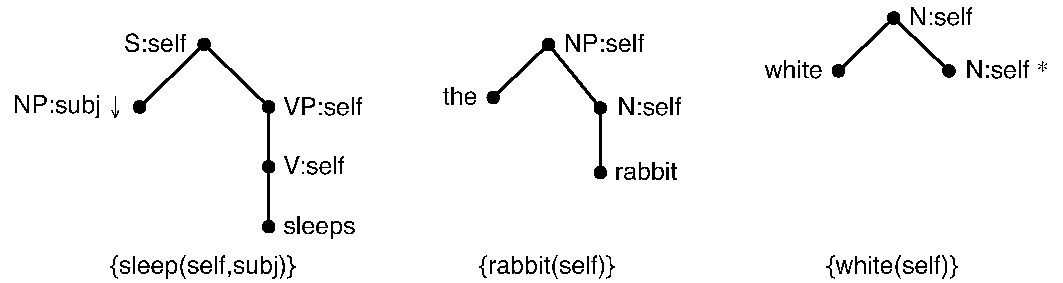
\includegraphics[width=\columnwidth]{pic-grammar}
  \caption{The example grammar.}
  \label{fig:white-rabbit-sleeps-grammar}
\end{figure}

\begin{figure}
  \centering
  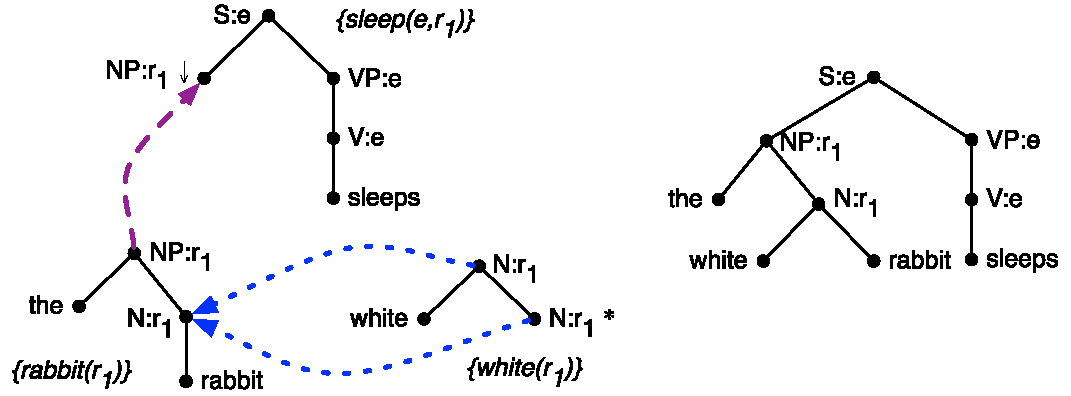
\includegraphics[width=\columnwidth]{pic-derivation}
  \caption{Derivation of ``The white rabbit sleeps.''}
  \label{fig:white-rabbit-sleeps-deriv}
\end{figure}

%\citeauthor{KolSto07}~\shortcite{KolSto07} attempt to improve the
%efficiency by translating the SPUD sentence generation problem into a
%planning problem and using a planning algorithm for generation.  We will
%now illustrate how they do this by a (simplified) example.

To improve on the efficiency of SPUD,
\citeauthor{KolSto07}~\shortcite{KolSto07} translate the sentence
generation problem into a planning problem and use a planning algorithm for
generation. We illustrate this process on a simplified example.

Consider a knowledge base containing the individuals $r_1$ and $r_2$, and a
set of attributes encoding the fact that $r_1$ and $r_2$ are rabbits, $r_1$
is white and $r_2$ is brown, and $r_1$ sleeps.  Say that we want to express
the information $\{\mathsf{sleep}(r_1)\}$ using the tree-adjoining grammar
shown in Fig.~\ref{fig:white-rabbit-sleeps-grammar}. This grammar consists
of \emph{elementary trees} (i.e., the disjoint trees in the figure), each
of which contributes certain \emph{semantic content}. We can instantiate
these trees by substituting individuals for \emph{semantic roles}, such as
$\mathsf{self}$ and $\mathsf{subj}$, and then combine the tree instances as
shown in Fig.~\ref{fig:white-rabbit-sleeps-deriv} to obtain the sentence
``The white rabbit sleeps''. The SPUD algorithm computes this grammatical
derivation by starting with the elementary tree for ``sleeps''. This tree
satisfies the need to convey the semantic information, but introduces a
need to generate a noun phrase (NP) for the subject, which also refers
uniquely to the target referent $r_1$. In a second step, SPUD substitutes
the tree for ``the rabbit'' into the open NP leaf, which makes the
derivation grammatically complete. Since there are two different
individuals that could be described as ``the rabbit''---technically, $r_2$
is still a \emph{distractor} (i.e., a \todo{one line definition here}) for
the referring expression---we are still not finished. To complete the
derivation, the tree for ``white'' is added to the existing structure by
the \emph{adjunction} operation, making the derivation syntactically and
semantically complete.


\begin{figure}[t]
\centering
{\small%
\begin{verbatim}
(:action add-sleeps
   :parameters (?u - node
                ?xself - individual
                ?xsubj - individual)
   :precondition (and (subst S ?u)
      (referent ?u ?xself)
      (sleep ?xself ?xsubj))
   :effect (and (not (subst S ?u))
      (expressed sleep ?xself ?xsubj)
      (subst NP (subj ?u))
      (referent (subj ?u) ?xsubj)
      (forall (?y - individual)
         (when (not (= ?y ?xself))
            (distractor (subj ?u) ?y)))))

(:action add-rabbit
   :parameters (?u - node
                ?xself - individual)
   :precondition (and (subst NP ?u)
      (referent ?u ?xself)
      (rabbit ?xself))
   :effect (and (not (subst NP ?u))
      (canadjoin N ?u)
      (forall (?y - individual)
         (when (not (rabbit ?y))
           (not (distractor ?u ?y))))))

(:action add-white
   :parameters (?u - node
                ?xself - individual)
   :precondition (and (canadjoin N ?u)
      (referent ?u ?xself)
      (rabbit ?xself))
   :effect (forall (?y - individual)
      (when (not (white ?y))
         (not (distractor ?u ?y)))))
\end{verbatim}}%
\caption{PDDL actions for generating the sentence ``The white rabbit
sleeps.''}
%\caption{Generating ``The white rabbit sleeps'' as a planning problem.}
\label{fig:white-rabbit-as-planning}
\end{figure}


The process described above has clear parallels to planning: we manipulate
a state by applying actions in order to achieve a goal. We can make this
connection even more precise by translating the SPUD problem into a
planning problem. For instance, Fig.~\ref{fig:white-rabbit-as-planning}
shows the corresponding PDDL actions for the above generation task, where
each action corresponds to an operation that adds a single elementary tree
to the derivation.  In each case, the first parameter of the action is a
node name in the derivation tree, and the remaining parameters stand for
the individuals to which the semantic roles will be instantiated.  The
syntactic preconditions and effects are encoded using $\mathsf{open}$ and
$\mathsf{canadjoin}$ literals; the status of each referring expression is
tracked using $\mathsf{distractor}$ literals. Notice that the action
effects contain terms of the form $\mathsf{subj}(u)$, which construct new
node names. In order to meet the syntactic requirements of PDDL, these
terms can be eliminated by estimating an upper bound $n$ for the plan
length, making $n$ copies of each action, ensuring that copy $i$ can only
be applied in step $i$, and replacing the term $\mathsf{subj}(u)$ in an
action copy by the constant $\mathsf{subj}_i$.

Once we've defined appropriate actions, we can solve the generation
problem as an ordinary planning problem. For instance, the following plan
solves our previous example:
%
\begin{enumerate}
\item $\mathsf{sleeps}(\mathsf{root}, r_1)$
\item $\mathsf{rabbit}(\mathsf{subj}(\mathsf{root}), r_1)$
\item $\mathsf{white}(\mathsf{subj}(\mathsf{root}), r_1)$
\end{enumerate}
%
Using this plan, the grammatical derivation in
Fig.~\ref{fig:white-rabbit-sleeps-deriv}, and therefore the generated
sentence, can be systematically reconstructed. Thus, we can solve the
sentence generation problem via the detour through planning and bring
current search heuristics for planning to bear on generation.



\subsection{Planning in instruction giving}

The object of the GIVE Challenge (``Generating Instructions in Virtual
Environments''; Koller et al.\ \citeyear{alexander07:_shared_task_propos})
is to build an NLG system which is able to produce natural-language
instructions which will guide a human user in performing some task in a
virtual environment. From an NLG perspective, GIVE makes for an
interesting challenge because it is a theory-neutral task that exercises
all components of an NLG system, and emphasizes the study of communication
in a (simulated) physical environment. It also has the advantage that the
user and the NLG system can be physically in different places, as long as
the 3D client and the NLG system are connected over a network. This makes
it possible to evaluate GIVE NLG systems on a large scale over the
Internet. The first GIVE evaluation will take place in late 2008;
currently eight research teams from five countries are working on
developing systems to participate in the challenge.\footnote{See the GIVE
 website for more details about this project:
 \url{homepages.inf.ed.ac.uk/v1akolle/proj/give/}.}

\begin{figure}
\centering
%\includegraphics[width=1 \columnwidth]{give_world_no_expl}
\includegraphics[width=1 \columnwidth]{give_world_2}
\caption{Map of the GIVE development world.}
  \label{fig:give-development-world}
\end{figure}

A map of an example GIVE world is shown in
Fig.~\ref{fig:give-development-world}.  In this world, the user's task is
to pick up a trophy in the top left room.  The trophy is hidden in a safe
behind a picture, so the user must first move the picture out of the way
and open the safe by pushing a sequence of buttons (the small square boxes
on the walls) in the correct order.  In order to get to all these buttons,
the user must also open the lower door and deactivate the alarm tile by
pushing further buttons.  To simplify both the planning and the NLG task,
the world is discretized into tiles of equal size; the user can turn by 90
degree steps in either direction, and can move from the centre of one tile
to the centre of the next. Some of the actions the user can take are shown
in Fig.~\ref{fig:give-planning}, in PDDL syntax.

\begin{figure}[t]
{\small%
\begin{verbatim}
(:action move
   :parameters (?from - position
                ?to - position
                ?ori - orientation)
   :precondition (and (player-pos ?from) 
      (adjacent ?from ?to ?ori) 
      (player-orient ?ori)
      (not-blocked ?from ?to)
      (not-alarmed ?to))
   :effect (and (not (player-pos ?from))
      (player-pos ?to)))

(:action turn-left
   :parameters (?ori - orientation
                ?newOri - orientation)
   :precondition (and (player-orient ?ori)
      (next-orient-left ?ori ?newOri))
   :effect (and (not (player-orient ?ori))
      (player-orient ?newOri)))

(:action turn-right
   :parameters (?ori - orientation
                ?newOri - orientation)
   :precondition (and (player-orient ?ori)
      (next-orient-right ?ori ?newOri))
   :effect (and (not (player-orient ?ori))
      (player-orient ?newOri)))

(:action manipulate-b1-off-on
   :parameters (?pos - position)
   :precondition (and (state b1 off)
      (player-pos ?pos)
      (position b1 ?pos))
   :effect (and (not (state b1 off))
      (state b1 on)
      (not (state d1 closed))
      (state d1 open) 
      (not (blocked pos_6_5 pos_6_4))
      (not (blocked pos_6_4 pos_6_5))))
\end{verbatim}}%
\caption{PDDL actions for the GIVE domain.}
\label{fig:give-planning}
\end{figure}

The plans generated in the GIVE domain are often nontrivial. For instance,
in the example above the shortest plan consists of 108 action steps; the
first few steps are as follows:
%
\begin{enumerate}
\item $\mathsf{turn}\textsf{-}\mathsf{left}(\mathsf{north}, \mathsf{west})$
\item $\mathsf{move}(\mathsf{pos\_5\_2}, \mathsf{pos\_4\_2}, \mathsf{west})$
\item $\mathsf{manipulate}\textsf{-}\mathsf{b1}\textsf{-}\mathsf{off}\textsf{-}\mathsf{on}(\mathsf{pos\_5\_2})$
\item $\mathsf{turn}\textsf{-}\mathsf{right}(\mathsf{west}, \mathsf{north})$
\end{enumerate}
%
(Most of the actions in this plan are ``move'' actions.) The bulk of the
GIVE problem can be considered a variant of the Gridworld problem, which
also involves finding a route through a world with discrete positions---but
with the additional need to press buttons in the right order, reason about
many more objects in the world, and navigate somewhat more complicated room
shapes.

The task of generating natural language instructions in this domain is also
more complicated than just a straightforward translation of the action
steps in a plan. For instance, the NLG system could generate an instruction
sequence starting with ``turn left; walk forward; press the button; turn
right; walk forward; walk forward; turn right; walk forward; walk forward;
turn left; walk forward''.  However, this would be clumsy and boring, and
it is to be expected that frustrated users will quickly cancel an
interaction with such a system, resulting in a bad evaluation score.
Having just pressed the button, it would be much better to say ``turn
around and walk through the door''.  This means that the mapping from
action instances to natural language instructions is not trivial.
Conversely, it may also be necessary to express a single planning step with
several instructions.  Having just entered the top left room, it may be
easier for the user to understand the instruction ``walk to the centre of
the room; turn right; now press the green button in front of you'' than the
instruction ``press the green button on the wall to your right''.  To plan
the referring expression ``the green button in front of you'' at a time
when the button is not yet in front of the user, the NLG system must keep
track of the hypothetical changes in what objects are visible to the user.
Thus the acts of referring and instructing, and the modules for planning
and NLG, must be tightly integrated.

Plan execution monitoring also plays an important role in the GIVE problem.
At a high level, the system needs to monitor a user's actions and compare
them against the generated instruction set to determine if the user has
correctly followed directions or not. In the case of the latter, new
instructions may have to be generated. In practice, the situation
can be quite complicated since the mental state of the user is not known
and so the system must observe the user's actions in real time. For
example, a user directed to ``turn around and walk through the door'' may
not necessarily perform these actions to the letter, i.e., immediately
turning 180 degrees and proceeding directly to the door. Instead, the user
might take a roundabout route through the room, eventually exiting out the
door. Although the user's actions do not match the generated instructions
exactly, they meet the intended goal. The system must be able to identify
such ``equivalent'' plans and not immediately generate new instructions as
soon as the user's actions have gone off course. Furthermore, a user can
communicate certain intentions to the system, both through action and
inaction. For instance, the system may correctly infer that a user has
failed to follow instructions if the user exits a room when given a
directive to ``walk to the centre of the room''. However, the system should
also be able to make a similar conclusion if a user simply does nothing
when given the instruction. Thus, such real-time plan monitoring is
essential in the GIVE domain, and also affects other modules in the system.


%%% Local Variables: 
%%% mode: latex
%%% TeX-master: "experiences"
%%% End: 
